% header.tex

% title on top of the document


% Main content
\newcommand{\headerinfo}{%
	%\vspace{-2cm}
	\maintitle{Adithya Balaji}
	\vspace{0.4em}\\
	\textsmaller{+}1 (919)--656--2815\sbull{}
	\href{mailto:adithyabsk@gmail.com}{adithyabsk\mbox{}@\mbox{}gmail.com}\sbull{}
	\href{https://github.com/adithyabsk}{github://adithyabsk}\sbull{}
	\href{https://linkedin.com/in/adithyabsk}{linkedin://adithyabsk}
	\vspace{0.4em}\\
	Raleigh\sbull{}
	North Carolina\\
	\vspace{1.5em}%
	\emph{\footnotesize Please see \href{http://www.linkedin.com/in/adithyabsk}{Adithya's LinkedIn profile} for more experiences/references.}
}

% \null \vfill make sure that the image is centered with the multicols text
% Modify columnsep to accomodate image and set back to default value
\newcommand{\headercontent}[3]{%
	\iftoggle{hideimage}{%
		\headerinfo{}\spacedhrule{0.8em}{0.8em}
	}{%
		\setlength{\columnsep}{-44em}
		\vspace{#1}%
		\begin{multicols}{2}
			\hspace{#2} % remove some variable space if single column
			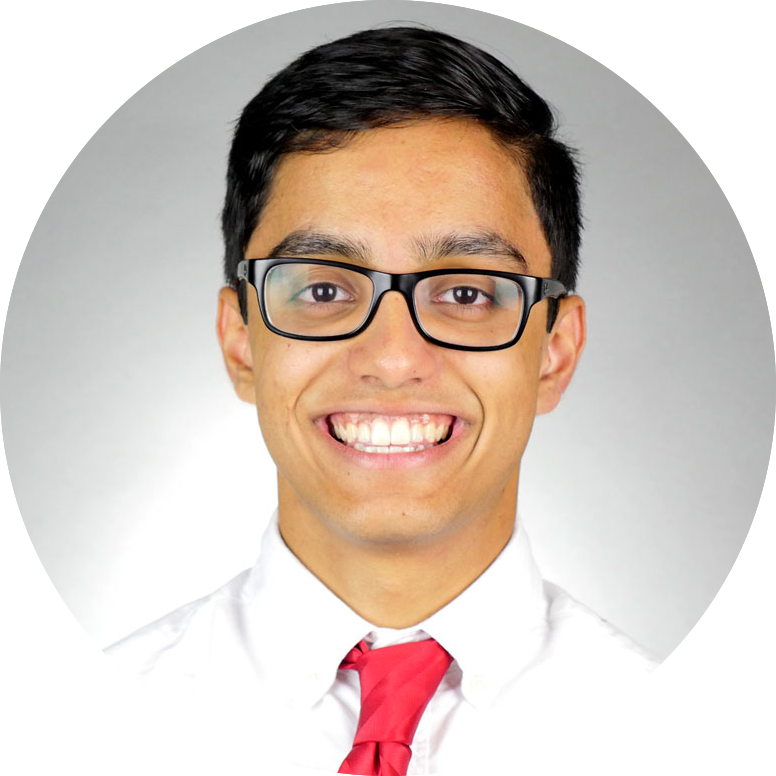
\includegraphics[width=2cm]{headshot}
			\vfill\null\columnbreak{}
			\headerinfo{}
		\end{multicols}
		\setlength{\columnsep}{10pt}\spacedhrule{-1.2em}{#3}
	}
}

% Some serious space hacking was necessary to make the header remain
% constant between twocols and not twocols
\makeatletter%
\if@twocolumn%
	\twocolumn[
		\headercontent{-0.4cm}{0cm}{0.8em}
	]
\else% \@twocolumnfalse
	\headercontent{0em}{-0.55cm}{-0.6em}
\fi
\makeatother
